\documentclass[runningheads]{llncs}
\usepackage{graphicx}
\usepackage{amsmath,amssymb} % define this before the line numbering.
\usepackage{ruler}
\usepackage{color}
\usepackage[caption=false]{subfig}
\usepackage{lipsum}
\usepackage[width=122mm,left=12mm,paperwidth=146mm,height=193mm,top=12mm,paperheight=217mm]{geometry}
\usepackage{hyperref}

\graphicspath{{figures/}}

\begin{document}
% \renewcommand\thelinenumber{\color[rgb]{0.2,0.5,0.8}\normalfont\sffamily\scriptsize\arabic{linenumber}\color[rgb]{0,0,0}}
% \renewcommand\makeLineNumber {\hss\thelinenumber\ \hspace{6mm} \rlap{\hskip\textwidth\ \hspace{6.5mm}\thelinenumber}}
% \linenumbers
\pagestyle{headings}
\mainmatter
\def\ECCV16SubNumber{14}  % Insert your submission number here

\title{Project Report for Panoramic Photo Generation}

%\titlerunning{ECCV-16 submission ID \ECCV16SubNumber}

%\authorrunning{ECCV-16 submission ID \ECCV16SubNumber}

\author{Yuanbo Han, %(u6617017),
Zhoubao Mai, %(u6118739),
Yujia Zhang, %(u6075459),
Ruiqi Zhou %(u5909724)
}
\institute{Paper ID \ECCV16SubNumber}

\maketitle

\keywordname{ key frame selection, scale invariant feature transform, random sample consensus, cylindrical projection, image blending}

\section{Introduction}

Panoramic photo generation is emphasized by the desire to get an overview of landscape and the restriction that camera's field of view is too small to be capable of capturing all-around view over the entire horizon. Thus, panoramic photography became popular in the 19th century \cite{luhmann2004historical}, and has been further promoted by the applications in computer vision and computer graphics nowadays. During the development of panoramic photography, swing lens and spherical fish-eye lens are invented successively \cite{deng2003generating}. Omni-directional camera is also utilized for panoramic photography while compromising image resolution \cite{nayar1997catadioptric}. The generation of digital camera deals with the shortcomings of these approaches, such as lens distortion and low resolution. Besides, there are existing studies of geometry modeling, camera calibration and feature matching. So, it is possible to explore a practical method to generate panoramic images from a simple digital camera and stitching methods, which is applicable for daily uses. This report demonstrates techniques for generating a cylindrical panoramic image based on an all-around video taken by an ordinary digital camera without wide-range capability. The procedure involves key frame selection, cylindrical projection, image registration, homography transformation and image wrapping, blending and cropping. A discussion is conducted based on the observation of the experiment results and potential future work.

\section{Related Work}

Many techniques have been proposed to solve image registration so that the panoramic image can be generated from an image sequence. These algorithms are illustrated chronologically, in which different levels of the feature are used for registration. Sequential Similarity Detection algorithms (SSDAs) compare image pixel values to deal with translational registration problem \cite{barnea1972class}. Correlation methods are employed to determine the similarity, and the sequential search would terminate before exhausted iteration on each pixel, reducing the computational complexity. However, SSDAs are not adaptive to magnification and rotation transformation. Therefore it has limited applications.

Image registration using features in the frequency domain is developed to solve translation and rotation in panoramic photography \cite{de1987registration}. Fourier transformations from the time domain to frequency domain are conducted on both images to be stitched together, then the ratio between them is calculated. Determination of rotation angle uses the form of this ratio in polar coordinates and simplifies it once appropriate rotation angle is found. Then the translation can be determined by phrase correlation methods. Fourier Transform has the corresponding counterpart for translation, rotation and scale, therefore has broad applications in image registration. Besides, Fast Fourier Transform provides an efficient solution.

Low-level features like corners or edges are referred to as control points and used to determine transformation functions in image registration \cite{goshtasby1988image}. Control points are selected based on their numeric features. In the application of panoramic photography, geometry distortion is inevitable. Thus, global transformation functions, e.g., least-squares method are inappropriate due to the insensitivity of a local property. Approximation methods are then proposed to register images with local geometric difference, including weighted least-squares and local weighted mean methods, meanwhile introducing much computation complexity. Therefore, the researchers carried out a practical image registration using the weighted least-squares method with orthogonal polynomial to reduce the equations to be solved.

A successful attempt to eliminate the restriction on motion parallax is introduced \cite{szeliski1997creating}. The Rotation matrix is utilized for image registration instead of cylindrical or spherical coordinates to solve singularity problems, meanwhile, ``gap closing'' technique is developed to deal with error accumulation. Degree of ``mis-registration'' can be obtained by calculating rotation matrices difference (quotient), and is converted into gap angle to update focal length after constructing the panoramic photography. Moreover, ``block adjustment'' is employed to update rotation matrix and focal length simultaneously for further optimization.


\section{Approach}

\subsection{Key Frame Selection}

Key frame selection and extraction are served as preprocessing for panoramic photography. VideoCapture object is created to capture the live stream from the video file and every frame is included in the stream \cite{opencv}. Hence, there is a large number of frames in the stream and these consecutive frames contain significant overlap with their neighbors. Stitching frames on the raw stream will be too time-consuming without acquiring noticeable information. In other words, the performance will be upgraded in many aspects if key frames can be extracted \cite{fadaeieslam2009key}. The first frame is chosen by default and the following frames are selected based on the number of matched descriptors between itself and the last selected key frame. Too many matched descriptors indicates the candidate frame is quite similar with the last selected one, thus cannot provide much progress for panoramic generation. On the contrary, if the two successively selected key frames have too few matched descriptors, the performance of feature detection is likely to be lessened in the next stage. In the implementation, upper bound and lower bound are prescribed for the number of matched descriptors to determine key frame selection. Only the frames of appropriate degree of overlap with the last selected frame would be extracted. Detecting areas are both two thirds of the total frames, because this is the fraction of the overlapping part over the entire canvas in experiment.

\subsection{Feature Detection and Matching}

Features are detected and matched between adjacent key frames to estimate homography matrix, which is used for image wrapping in the next procedure. Since key frames can be captured in different views, a reliable matching method should depends on invariant feature extraction. Scale Invariant Feature Transform (SIFT) is proposed to extract local features that are invariant to image scale, rotation and change in 3D viewpoint \cite{lowe2004distinctive}. Four stages are implemented accordingly in SIFT algorithm. Scale-space extrema detection uses Difference-of-Gaussian to search local features in different locations with different scales, leading to the extracted feature invariant of scale and location. Key point localizations and orientation assignments assign the locations, scales and orientations of the candidate key points, which are used in the descriptors to guarantee transformation invariance. Keypoint descriptor is generated to describe local image gradients, so it is highly distinctive.

Feature matching is carried out based on these key points and descriptors. Brute-Force matcher computes L2 distance (Euclidean distance) exhaustively between all feature vectors from both images and find the pairs of descriptors that have the smallest distance. To eliminate false-positive in the raw match from Brute-Force matcher, David Lowe's ratio (which is 0.6 in the implementation) is used to select valid match, whose distance is less than 0.6 times the distance of the second best nearest neighbor. Example of key points' matching is illustrated in Fig.~\ref{fig:sift1}.

\begin{figure}[h!]
  \centering
  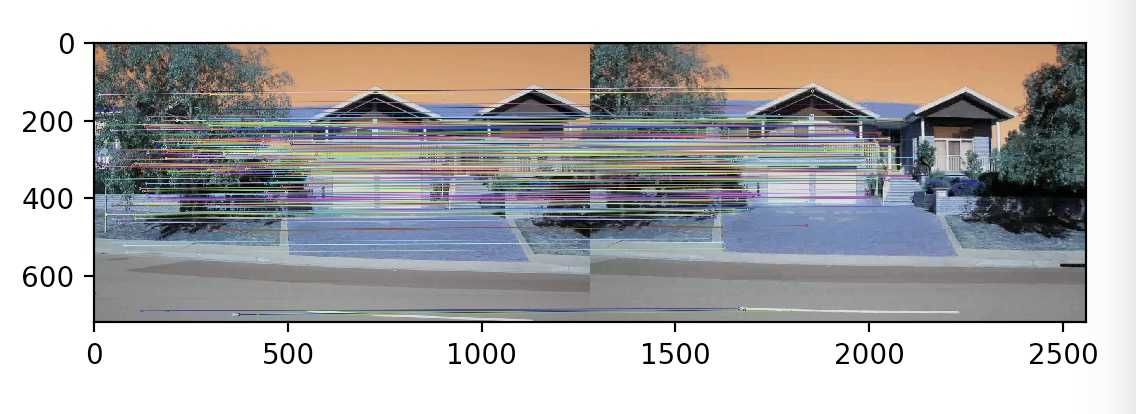
\includegraphics[scale=0.6]{sift1.jpg}
  \caption{Example of SIFT Matching}
  \label{fig:sift1}
\end{figure}

However, it is not easy to find a proper David Lowe's ratio. When increasing the ratio, there will be lots of mismatched points. When reducing the ratio, the number of mismatched points will decrease, but so is the number of matching points. One way to deal with this problem is to find a robust estimation method to eliminate the mismatches. In practice, Random Sample Consensus (RANSAC) algorithm is applied to classify the correct matching points from mismatches. As a matter of fact, there is great robustness in RANSAC algorithm including the ability to handle sparse and multiple structured data.

\subsection{Image Wrapping}

Given the homography matrix $\mathrm{H}$ derived from the matched feature vectors, stitch new frame to the image composed of previous frames, until finally the panoramic image is accomplished. Since using planar homography will result in a vertical distortion if the rotation angle of camera is above 120 degrees, a cylindrical projection should be applied to the new key frame before computing homography matrix. As the project assumes the camera is level and only rotates around the vertical axis, images only need translation transform after applying cylindrical projection. The formula for cylindrical projection is shown below, where the cutting-point of the cylindrical plane and flat plane is the origin point. x$_{p}$ and y$_{p}$ represent planar coordinates, $x_{c}$ and $y_{c}$ represent cylindrical coordinates respectively, $f$ is the focal length of camera, and $\alpha$ is the angle between the line from cylinder center to the cutting-point and the line from cylinder center to the examining point.

\begin{gather}
  \alpha =\arctan\frac{x_p}{f} \\
  x_c = f \alpha \\
  y_c = y_p \cos\alpha
\end{gather}

A cylindrical projection is applied in reverse interpolation. To get pixel value of each point in cylindrical coordinates, calculate the corresponding planar coordinates and get its pixel value to fill the cylindrical plane. Reverse interpolation guarantees every pixel in the projected image has corresponding intensive value.

SIFT descriptors are used to match the new frame that has been projected to the cylindrical plane and the image with previous frames. If the valid match has more than four pairs of corresponding matching points, estimate parameters in homography matrix by RANSAC algorithm. Because it detects final inliers with the appropriately refined homography \cite{wu2007improved}. Transform the original images based on the homography matrix to wrap them onto the common image surface, and concatenate them accordingly to build the final panoramic result. The successive merged results are displayed in Section~\ref{sec:result}.

Focal length in the camera is adaptive during shooting, and this parameter influences the result of cylindrical projection. Besides, various light conditions in different frames as well as auto exposure settings of the camera, which is a usual case by default, also result in some discontinuities in the stitching result.

\subsection{Blending and Cropping}

The distortions and discontinuities in the stitching result should be alleviated by blending and cropping in the last procedure. Illuming difference leads to visible seams in the panoramic image, so various approaches to image blending have been tested in this implementation to achieve smooth transition. Linear blending has the advantage of easy implementation and fast executing, weighted average method works on pixel values in the overlapping area \cite{li2008automatic}. The result is illustrated in Fig.~\ref{fig:linear}, in comparison to the above image without blending.

\begin{figure}[h!]
\centering
\subfloat[Without blending]{%
  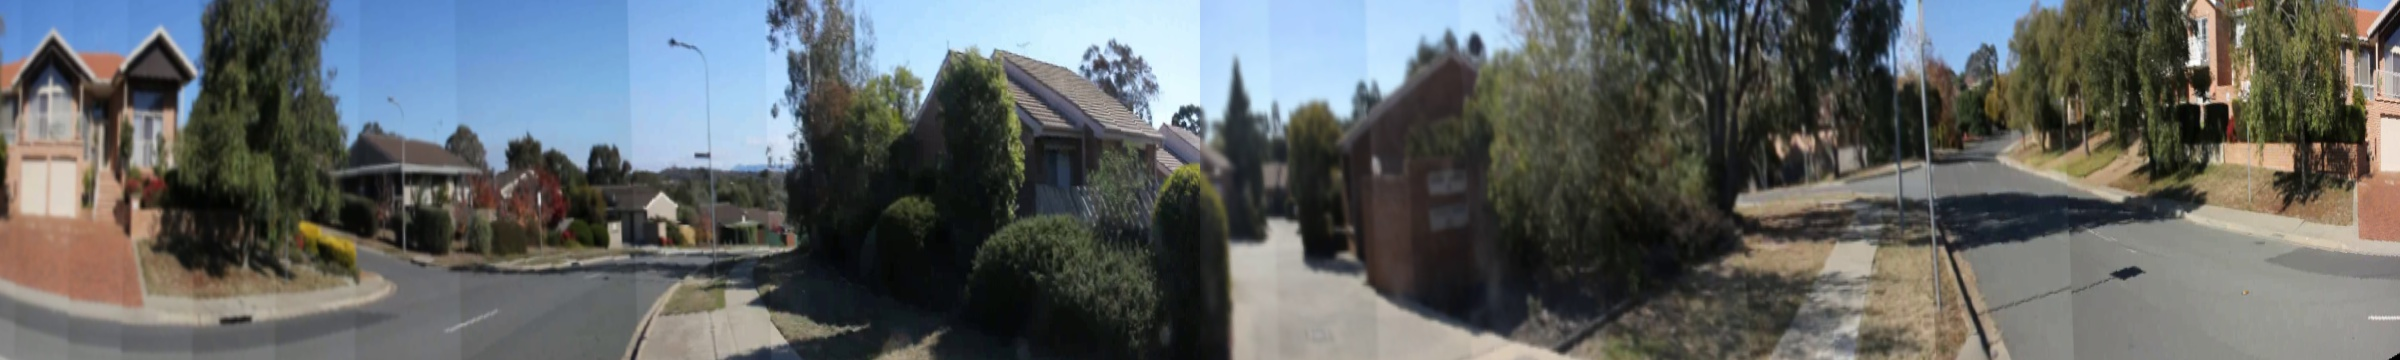
\includegraphics[width=\linewidth]{panoramic.jpg}%
}

\subfloat[Linear blending]{%
  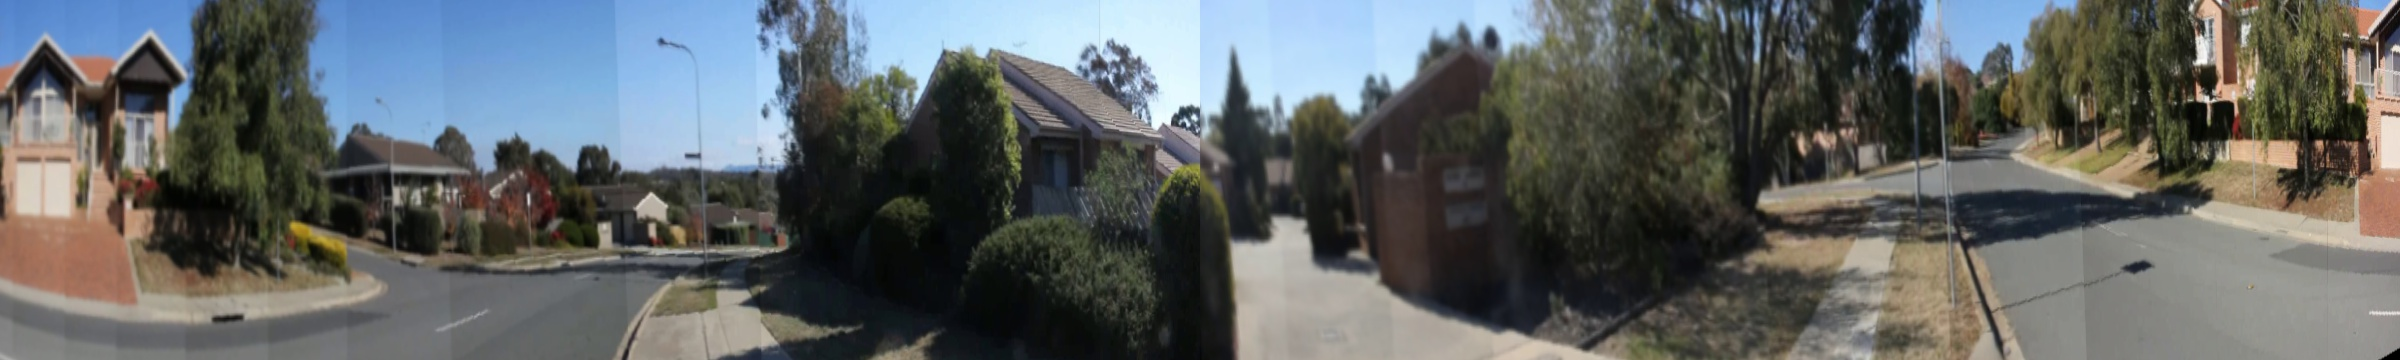
\includegraphics[width=\linewidth]{linear}%
  \label{fig:linear}
}

\subfloat[Laplacian blending]{%
  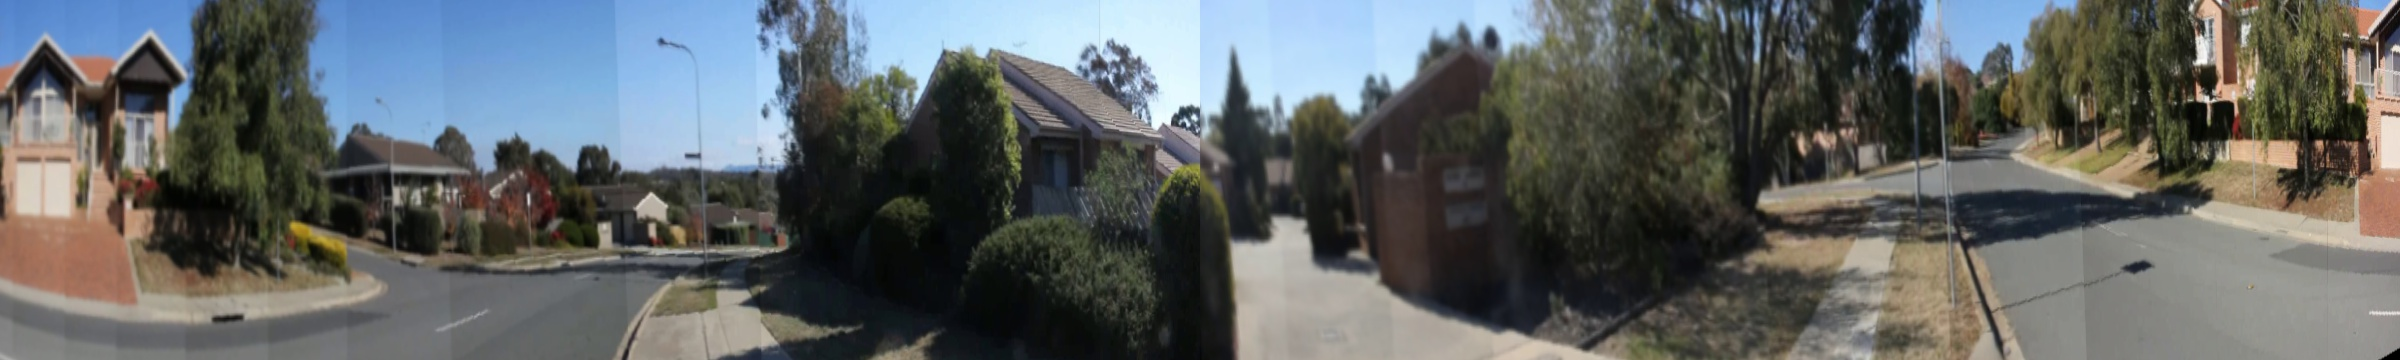
\includegraphics[width=\linewidth]{linear}%
  \label{fig:Laplacian}
}

\caption{Results for blending}
\end{figure}

As a result, the seams are less visible after linear blending. However, ghosting may appear where the same object appears twice in different positions \cite{juan2010surf}. Besides, there is a remaining problem for window size choosing, which refers to the transition zone or overlap area while blending. If the window size is small, there still exists visible step at the boundary of two neighbor frames. If the window size is big on the contrary, objects in the different images might appear superimposed, and therefore leads to ghosting artifacts.

Pyramid blending is also attempted to eliminate ghosting artifacts while alleviating color distortion. First, the images to be stitched together are decomposed into sets of band-pass filtered component images by a series of low-pass filters, which uniformly cover the range of frequencies in original image. Gaussian pyramids are constructed in that way, then differences of adjacent levels are used to construct corresponding Laplacian pyramids. A third Laplacian pyramid is developed by composing nodes from the same layer of two pyramids together by weighted average splining method. Finally, the levels in third pyramid which are band-pass images are summed up for the final joint result. The result is shown in Fig.~\ref{fig:Laplacian}. However, the outcome is not as ideal as that in \cite{burt1983multiresolution}. Possible reasons include inappropriate choice of mask for composition, or incorrect handling for bound conditions.

Cylindrical projection is implemented before image stitching, so irregular boundaries appear in raw output. To obtain rectangular boundaries for the panoramic image, cropping and other image completion techniques should be applied \cite{he2013rectangling}. Contour is derived from the original image and approximations of its rectangular shape determine the shape of final output.  The result is illustrated in Fig.~\ref{fig:cropping}, where the above image is the original panoramic photo without cropping, and the below one with cropping manipulation.

\begin{figure}[h!]
\centering
\subfloat[Without cropping]{%
  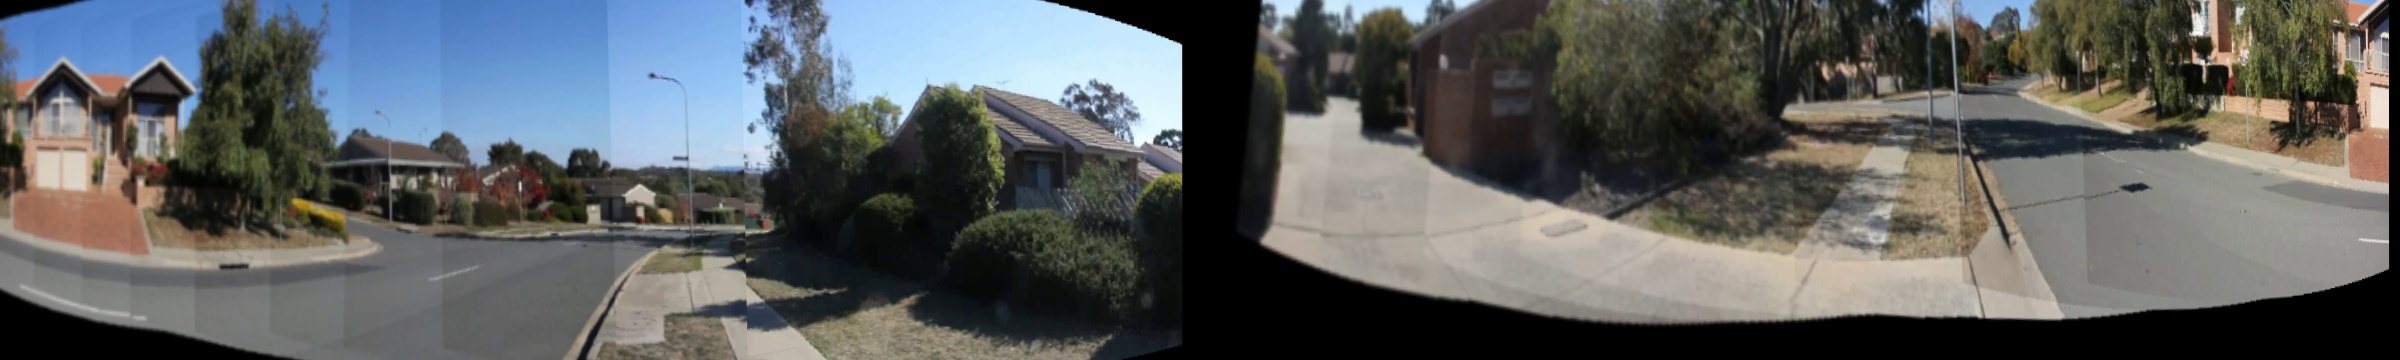
\includegraphics[width=\linewidth]{beforecropping.jpg}%
}

\subfloat[With cropping]{%
  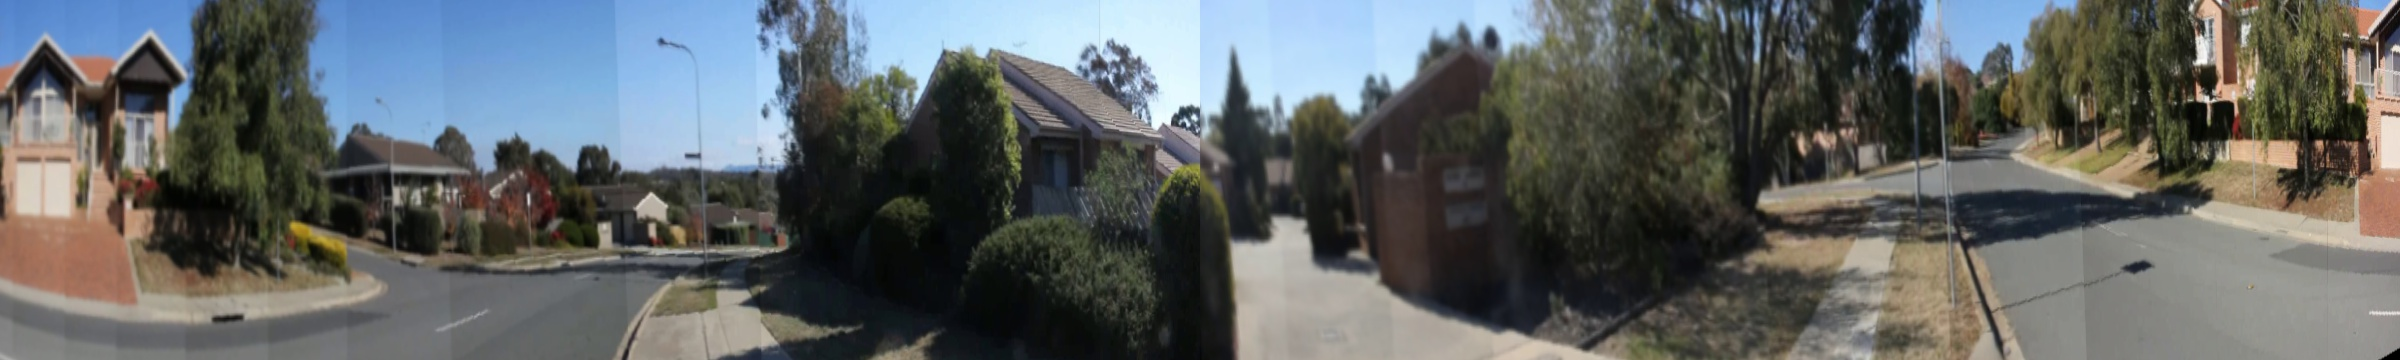
\includegraphics[width=\linewidth]{linear}%
}

\caption{Result for cropping}
\label{fig:cropping}
\end{figure}


\section{Experiment Outcome}
\label{sec:result}
The stitching procedure is shown in Fig.~\ref{fig:stitch}. The first image is the first frame captured by the camera. The next two images are intermediate results in image registration and stitching procedure. The fourth image is the final panoramic photo with all key frames joint together and after further optimization including histogram equalization for uneven exposure, blending for color distortion and cropping for irregular boundaries. The transition is rather smooth and artifacts like blurring and ghosting have been alleviated.

\begin{figure}[h!]
\qquad
\subfloat[First frame]{
  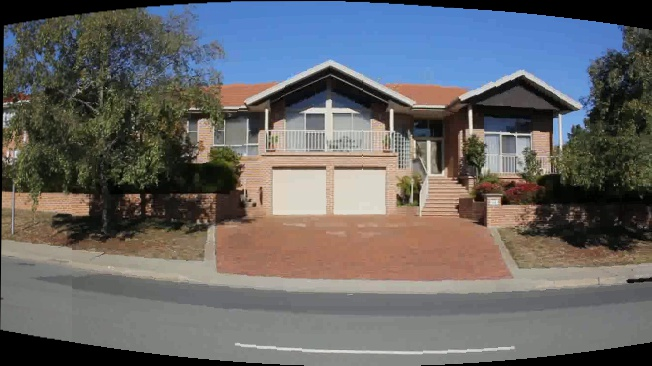
\includegraphics[scale=0.3]{result1}
}

\qquad
\subfloat[Image of stitching the first 3 frames]{
  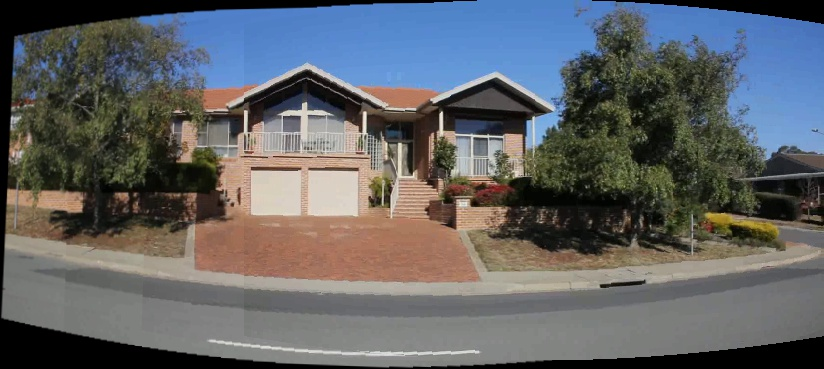
\includegraphics[scale=0.3]{result3}
}

\qquad
\subfloat[Image of stitching the first 5 frames]{
  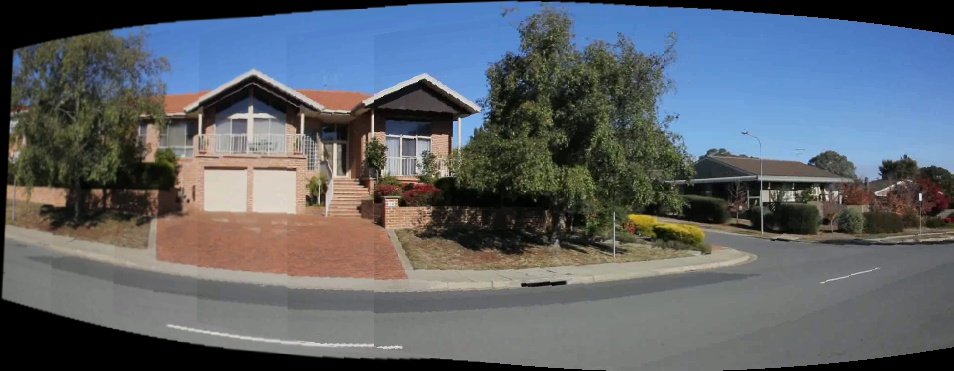
\includegraphics[scale=0.3]{result5}
}

\centering
\subfloat[Panoramic photo]{%
  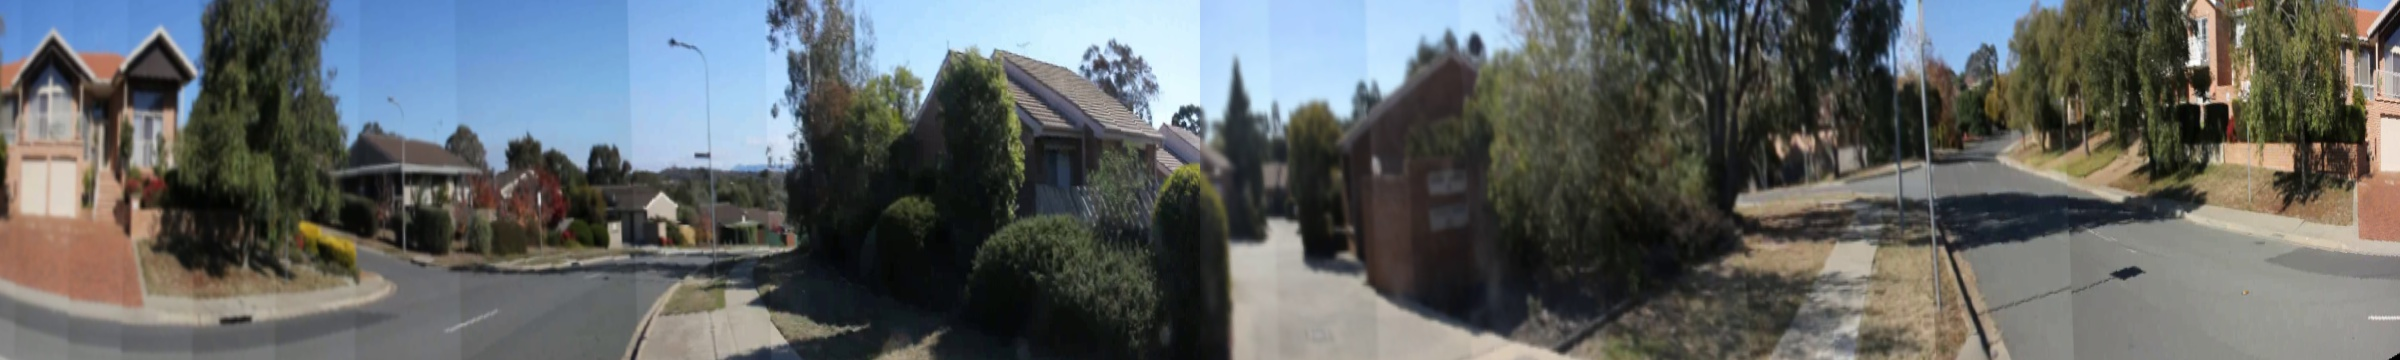
\includegraphics[width=\linewidth]{panoramic}%
}

\caption{Successive concatenate results}
\label{fig:stitch}

\end{figure}


\section{Conclusions}

Automatic panorama generation is proposed in this article, including key frame selection, feature detection, image registration, image wrapping, blending and cropping. The step-by-step results have been explained in previous sections. As a term project, team members grasp deeper understanding of image manipulation and practical techniques for this task.

There still exists potential work for further optimization to deal with the distortions and expansion of panoramic photography applications. PCA-SIFT can be implemented as an extension of SIFT with more distinctive local descriptors, and hence is more invariant to image deformations with higher accuracy \cite{ke2004pca}. The algorithm is similar with SIFT, where the salient aspects of the image gradient in the potential key points are encoded as descriptors. The extended part is that the normalization of gradient patch utilizes Principal Components Analysis (PCA). Experiment results illustrate the optimization in accuracy and matching speed.

Exposures are not even because the images are taken outdoor and the light conditions are changing constantly among these frames. In the implementation of this project, histogram equalization is used to handle the problem, but it is not entirely solved---the uneven exposure is still visible and influences blending results. One possible approach is Generalized Mosaicking, in which an optical filter with spatially varying properties is attached to camera \cite{schechner2003generalized}. The filter receives information in various lighting conditions, and the information builds new model to describe the conditions and achieves high dynamic range (HDR) mosaic. Integration of HDR radiance map and feathering technique guarantee that the procedure of generating panoramic photography will be invariant to uneven exposure to some extent \cite{jain2013review}.

Applications for panoramic photography can be extended to various areas. Motion analysis tasks like surveillance and smoke detection are time-consuming while employing complex equipments. Panoramic photography makes it possible to build omnidirectional monitoring system with small and compact devices to achieve optimal solutions \cite{kopilovic2000application}. Algorithm of generating panoramic photography could be utilized for dental panoramic X-ray to obtain tomographic image via wide X-ray beams \cite{arai1998dental}.


\section{Learning Outcome}

During the implementation procedure, we got familiar with the basic workflow of panoramic photo generation, including key frame selection, feature detection and matching, cylindrical projection, homography computation and image stitching. We also implemented related optimization techniques, such as blending for color distortion and cropping to correlate the final result. We reviewed literature on panoramic photography development and learned different approaches to achieve panorama generation. These methods utilize features of different levels, from pixel value, frequency domain, low-level features like edges to high-level features. Thereby, we were able to practice image manipulations on distinct levels and various perspectives. Further discussion and potential work inspired us to learn the cutting-edge techniques to solve the problem and extensive application scenarios for panoramic photo generation.


\bibliographystyle{splncs}
\bibliography{egbib}

\end{document}
